\documentclass{report}
% need it in .docx form? no problem!
% pandoc -s chapter-3.tex -o chapter-3.docx --bibliography="chapter-3.bib"; mv chapter-3.docx ~/Desktop

\usepackage{import}
\import{../}{gov-style}
\addbibresource{chapter-3.bib}

\begin{document}
\begin{refsegment}

\section*{Thesis so far}
\begin{em}
In this thesis, I seek to understand why nation-states (and the United States in particular) have not responded more harshly to cyber-espionage and whether that is likely to change. While the US acts diligently to prevent digital invasions, the punishment it inflicts on states for hacking into its computer networks and attempting to steal state secrets seems mild in comparison to the damage done. I theorize that this puzzling response to cyber-attacks can be explained by espionage norms that formed during the Cold War---norms that suggest a state will never extend the diplomatic consequences of an espionage attempt beyond the countermeasures necessary to prevent it. To make this connection, I will demonstrate the various forms in which this norm existed during the Cold War, then analyze how it influences our cybersecurity policy today.

In the last chapter, I described the evolution around early norms of aerial reconnaissance. I demonstrated how in response to a series of incredibly provocative overflight operations and numerous shootdowns of US aircraft, both the US and the USSR opted to downplay the significance of these incidents, and worked to resolve them with minimal diplomatic consequences and no military escalation. In this chapter, I will give an overview of the world of espionage that we know from popular culture---spies and human intelligence (HUMINT)---and demonstrate how even the most damaging espionage operations result in consequences no more severe than tit-for-tat diplomatic expulsions.
\end{em}

\section{Introduction}
The United States was the last major country in the world to establish an independent civilian intelligence service.\footcite[p.~35]{olson_fair_2006} Even after the success of the Office of Strategic Services (OSS) in WWII, Truman was still highly skeptical of a permanent civilian intelligence service. Reluctantly, he created the CIA in 1947, of which a third of the original employees were former OSS members.\footcite[p.~37]{olson_fair_2006} In an effort to ensure that the character of the intelligence service would be different from that of military intelligence, the initial command structure of Central Intelligence was dominated by the State Department.\footcite{troy_truman_1993}

Meanwhile, the Soviets exited World War II with perhaps the most formidable intelligence service in the world. The London \emph{rezident},\footnote{The chief spy at an embassy. In the US, they would be known as a ``station chief.''} Nikolai Rodin, boasted that no one could match the network of agents that Moscow had created there.\footcite[p.~151]{haslam_near_2015} And the Soviets had swiftly and successfully stolen one of America's most treasured wartime secrets, crucial information about the atomic bomb. When Truman first told Stalin that the Americans ``had a new weapon of unusual destructive force'' at the Potsdam conference in 1945, Stalin seemed ``neither surprised nor the least curious \textelp{} He did not, in fact, appear at all interested.''\footcite[p.~443]{mccullough_truman_1992}  Stalin's reaction was so off-putting that observers in the room wondered if he had even grasped the significance of what he'd been told. Apparently no one considered that Stalin already knew about the atomic bomb through several highly paced British and American spies in the Manhattan project, and that the Soviets had been running their own nuclear program since 1942.\footcite[p.~443]{mccullough_truman_1992}

Not only was the United States late to the game in setting up postwar intelligence operations, they were also at a structural disadvantage. With aerial reconnaissance a crucial asymmetry was at play---NATO allies had bases adjacent to Russian territory from which the US could launch flight missions, but the Soviets had no allied territory in the Western Hemisphere from which to do the same. The inverse advantage applied in the area of human intelligence. Soviet Russia was a deeply paranoid and isolated state, and Western intelligence services faced a number of challenges running agents there. Every Western diplomat was placed under round-the-clock surveillance and significant travel restrictions, making it difficult to contact and turn potential agents. The USSR operated the world's most effective secret police, and Soviet citizens were told to be suspicious of foreigners.\footcite[p.~42]{richelson_american_1987} In 1943, the official State Department recommendation was simply to avoid undercover activity altogether.\footcite[p.~44]{richelson_american_1987}

In my study of human intelligence, I will focus primarily on Soviet operations against the US and its allies. In part this decision reflects the natural advantage of the Soviet Union in the field of Human Intelligence---they had more opportunity to run agents in the US government, and so we have more opportunity to examine the cases where they did. But I also want to make sure that, in investigating how states respond to uncovering espionage, I balance which side is doing the spying. In order to be effective, a norm has to cut both ways. So while the last chapter exclusively discussed reconnaissance performed on the USSR by the United States, this chapter will apply the norm of limited diplomatic response to situations where, more often than not, the US was on the defensive.

The purpose of the thesis to argue that the same norm downgrading the severity of aerial reconnaissance holds true for all forms of espionage. Therefore, this chapter will examine that norm in the context where it is most well-developed---human spies. In the first section, I will show how the scholarship on this issue has evolved from initially regarding peacetime espionage as illegal (or at least taboo) to a tacit universal understanding that espionage is permitted, provided the perpetrating state is willing to accept that they cannot protect their spy from domestic prosecution. In the second, I will use publicly-available information about unmasked spies to demonstrate the sheer volume at which these operations are conducted, essentially without discouragement. And lastly, I will look at some of the most infamous, damaging spy cases and qualitatively discuss the responses of the states involved. In doing so I further my larger argument that the consequences of espionage, in all its forms, are upper-bounded.

\section{Legality of espionage}
\subsection{The basic arguments}
In addition to the capability difference, there is a key philosophical difference between human spies and aerial espionage: in the case of planes, the ``wrongness'' of violating a territorial boundary violation is extremely intuitive. The impermissibility of sending hostile military forces across a border line is foundational to the ontology of a nation-state and international legal conceptions of sovereignty.\footnote{I feel compelled to note that this is not the same as saying ``without borders with we have no nation'' in defense of restricting immigration, an argument which, regrettably, has some political currency today. Accommodating immigrants and refugees---stateless populations seeking to naturalize---is fundamentally different from being unable to repel invaders aligned with a hostile nation-state.} That hostilities did not substantively escalate after consistent American violations of this principle says something about how these flights were understood. It tells us that signaling a flight's purpose is peacetime espionage, even when from a military plane, is a distinction powerful enough to supersede our gut reaction that sending uninvited bombers into hostile territory constitutes an act of war.

The practice of spying is a little more complicated. It's clearly wrong, in the sense that treason and espionage are punished harshly under pretty much every legal code imaginable. In many countries it is an unforgivable sin, where even falling under suspicion can lead to imprisonment, torture, and death. While the latter two are sometimes criticized on human-rights grounds, no one disputes the right of a nation to punish those who work against them in service of a foreign power. Legally, as you will see in a moment, spies are essentially enemy combatants who are afforded none of the customary protections typically given to soldiers. The nation that sends a spy into a foreign country explicitly asks them to commit crimes on their behalf, and the spy risks paying the full price, all by themselves, if they are caught committing them.

Despite the fundamental illegality of espionage, it is possible that you already sort of feel like you know why countries don't punish each other more harshly for sending the spy in the first place. Please for the moment forgive my lack of scientific rigor, in service of a broader point---everyone understands that their government will be performing some undercover intelligence activities in foreign countries. We generally hope that our government is using the appropriate discretion in choosing to undertake these missions we know nothing about, and expect that they are defending against those attempts by others. That national governments will attempt to collect and keep some state secrets is, in its barest form, a relatively noncontroversial premise.

The public level of comfort with the nature and scale of these secret activities naturally varies, especially in liberal democracies with a free and functional press. Daniel Ellsberg's decision to release the Pentagon Papers in 1971 precipitated the first in a series of scandals that plagued the CIA during that decade---electoral interference in Chile, domestic spying on antiwar activists, and complicity in Watergate all contributed to widespread distrust of American intelligence operations.\footcite[p.~214-215]{andrew_missing_1984} In 1975-6, Jimmy Carter explicitly campaigned for president on a promise to reign in the independence and abuses of American intelligence agencies.\footcite[p.~217]{andrew_missing_1984} Ronald Reagan would later unseat Carter with a promise to restore those capabilities, only to later find himself embroiled in his own covert action scandal, when senior administration officials and the CIA were implicated in the Iran-Contra affair.

And yet even with occasional resistance from the American public to covert activities abroad, the basic premise that the Federal Government should conduct espionage on other countries is always left unquestioned. At the height of anti-CIA sentiment in the '70s, Congress passed the Hughes-Ryan Amendment, which was intended to restore the CIA's original conception as an agency for intelligence only.\footcite[p.~215]{andrew_missing_1984} The Amendment prohibits CIA funds from being used for any activities other than ``activities intended solely for obtaining necessary intelligence.'' Hughes-Ryan and the Intelligence Oversight Act of 1980 are the only major pieces of legislation that curtailed CIA independence for the entire Cold War, spanning 1947-1991.\footcite[p.~93-94]{cogan_covert_1993} Both reaffirm the basic necessity of espionage and intelligence service, by contrasting ``good'' foreign intelligence gathering with ``bad'' covert action and interference.

By demonstrating that peacetime espionage is functionally legal, it might seem that I run the risk of undercutting my own premise. After all, if espionage is perfectly fine, then why would it be unusual that states choose not to escalate it? I offer two answers. The first is that I'm not trying to prove that state behavior is or is not unusual---I'm just trying to prove that it is a certain way, and that we can apply it in a range of scenarios. Second, when international law is codified, it generally emerges as a reflection of state practice.\footcite[p.~628]{sulmasy_counterintuitive_2007} In a few limited cases, it can rise to the level of \emph{jus cogens}---a peremptory norm that arises from some fundamental principle---but that is reserved for cases like slavery or genocide, offenses that are orders of magnitude more severe than spying.\footcite[p.~629]{sulmasy_counterintuitive_2007} Most times, international law is reactive, not normative. If international practice seems to permit espionage, it is because the international community has tacitly agreed to leave it that way, not because a higher power or principle decided so. Thus, my question is simply why states have decided that peacetime epsionage should be legal in the first place.

In the previous chapter, I argued that the US policymakers, all the way up to the President, sought to make clear a distinction between military flights and those of a ``spy plane.'' They hoped to invoke a nascent norm that treated peacetime espionage as something less serious than a military violation of sovereignty. Over the course of the Cold War, that norm would develop into an established series of state practices which, despite their remarkable consistency, are rarely acknowledged by those in power. Instead, peacetime espionage occupies an intentional liminal space in the international legal regime, where it can be simultaneously un-endorsed and unpunished.

\subsection{Wartime espionage}
How to classify a spy? If we think of spies as enemy combatants, then it would be simple to argue that running agents constitutes a flagrant violation of national sovereignty. There is precedent for this: during times of war, spies are, in fact, a special class of combatant. The Hague Rules of 1907 and the Geneva Convention of 1949 both have guidelines outlining the limited permissibility of espionage during wartime, and the proper conduct for when a spy is apprehended.\footcite[p.~652]{beim_enforcing_2018} The former defines a spy this way:

\begin{quote}
A person can only be considered a spy when, acting clandestinely or on false pretenses, he obtains or endeavors to obtain information in the zone of operations of a belligerent, with the intention of communicating it to the hostile party.

Thus, soldiers not wearing a disguise who have penetrated into the zone of operations of the hostile army, for the purpose of obtaining information, are not considered spies. Similarly, the following are not considered spies: Soldiers and civilians, carrying out their mission openly, entrusted with the delivery of dispatches intended either for their own army or for the enemy's army. To this class belong likewise persons sent in balloons for the purpose of carrying dispatches and, generally, of maintaining communications between the different parts of an army or a territory.

A spy, taken in the act, shall not be punished without previous trial.

A spy who, after rejoining the army to which he belongs, is subsequently captured by the enemy, is treated as a prisoner of war, and incurs no responsibility for his previous acts of espionage (Articles 29-31).\footcite{noauthor_hague_1907}
\end{quote}

Though a bit dated, the Hague convention is routinely cited as a starting point for discussions about the legality of espionage, and as a description of an intelligence operative acting improperly in a foreign country, it works nicely. The problem with this definition is that its primary purpose is to distinguish between an enemy spy and an enemy soldier. Without a war there are no belligerents and no soldiers, so what is left with which to define a spy? In the United States---a country that has not issued a Declaration of War since 1942---it is not entirely clear under what circumstances the rules of wartime espionage would apply at all.\footcite{ncc_staff_when_2018}

For our purposes, we can put aside the question of wartime espionage in the same way that University of Chicago Law Professor Quincy Wright does in a 1962 essay on this subject: if one takes the position that hostilities between the US and the USSR are sufficient to constitute a ``hot war,'' or that international law is always illusory, then the legality of espionage is irrelevant.\footcite[p.~8]{wright_espionage_1962} With the benefit of hindsight, neither of those propositions are true, so we can take it for granted that the US and the USSR were not at war, and the espionage that takes place between them is peacetime espionage.\footnote{I recognize that how to categorize the level of hostility in the Cold War is open to debate, as is the relevance of international law to states' actions. But however ``hot'' you think the Cold War really was, it clearly did not rise to the level where wartime rules about espionage would apply, and the only tool with which we have to evaluate the permissibility of peacetime espionage is international law.}

\subsection{Cold War debate about peacetime espionage}
The aforementioned essay by Professor Wright is part of a series of essays that to the best of my knowledge represent the first significant scholarly examinations of the legality of peacetime espionage. These \emph{Essays on Espionage and International Law} are interesting not only as a means to understand the evolution of scholarship historiographically, but also because they were published in 1962. At that time they were written, Gary Powers was still in a Russian prison, and US and Soviet policymakers were still grappling with how to respond to the new reality of constant, frantic intelligence-gathering efforts. In the two essays of the collection that deal directly with HUMINT, Wright and Julius Stone, a professor of International Law at the University of Sydney, offer competing arguments for whether peacetime espionage---with or without territorial incursion---is itself an international delinquency. Wright makes his case first, and Stone responds point-by-point---the first Valladolid debate of peacetime espionage.

Wright argues that peacetime espionage violates the principles of territorial integrity and political sovereignty. ``Any act by an agent of one state committed in another state's territory, contrary to the laws of the latter, constitutes intervention, provided those laws are not contrary to the state's international obligations.''\footcite[p.~13]{wright_espionage_1962} These are the same principles of territorial integrity that aerial reconnaissance violates, and as far as Wright is concerned, overflights are no different from human espionage. Both are unwanted incursions in space.

Since there are special wartime circumstances in which espionage is permitted, Wright allows for the possibility that such circumstances might be present in peacetime. He individually analyzes the US government's defenses of the U-2 overflights as general justifications for all forms of espionage.\footcite[p.~17. A fun question to ask yourself is whether putting human spies and overflights in the same category elevates the severity of human intelligence or minimizes that of overflights. I think it actually does both, and Wright seems to agree. An overflying plane is clearly capable of greater physical destruction but ``the difference should not be exaggerated. Although a reconnaissance airplane may carry bombs, a secret agent may plant a bomb and engage in various forms of sabotage.'' (p. 21) The general lack of concern that a spy plane might be carrying bombs is consistently surprising to me. Many of these flights were in retrofitted bombers, completely indistinguishable to enemies from their heavily-armed counterparts. Nonethless, both sides seem willing to treat reconnaissance flights as their own separate thing, and that protection applies to spies as well. As long as spies \emph{don't} engage in sabotage, the fact that they have the potential to do so is irrelevant.]{wright_espionage_1962} Most of these defenses come from the same general sentiment: everyone is doing it, and for our security we must as well. Wright is sympathetic, but after considering the different ways that states might spy on or interfere with each others' affairs, concludes that ``under present circumstances, it does not appear that a general rule justifying counter-intervention is expedient. Rather, action should be taken through the United Nations to terminate the original intervention.''\footcite[p.~22]{wright_espionage_1962} None of this is justified, and it should be curbed through international judicial means.

Raising the issue of espionage in the United Nations is a plausible option. You might remember from the last chapter that Eisenhower actually brought the shootdown of a Navy plane in front of the UN in 1954, but that a UN resolution was the response chosen precisely because all parties involved understood that it would be ineffectual. Eisenhower hoped to placate the American public outraged about the casualties, while at the same time avoid punishing the Soviets who (arguably) responded appropriately to American espionage efforts. In practice, most states dodge international law entirely by simply disowning their spies. This is how Wright describes the status quo in 1962: ``Since the government responsible \textelp{} seldom acknowledges its responsibility but allows the agent, if caught, to be punished without protest, such incidents are not usually the subject of international discussion.''\footcite[p.~15. As an argument for not invoking international law, I acutally find this a bit silly. Just because a bank robber never flips on their co-conspirators does not mean those co-conspirators cannot be indicted for their role in committing the crime.]{wright_espionage_1962}

Professor Stone's view is that the only thing illegal about espionage comes from the ancillary territorial violations that sometimes make it possible, not the espionage itself. Where Wright sees the disowning of spies as evidence of espionage's illegality, Stone sees it as a \emph{de facto} endorsement. ``Surely if espionage were a state delinquency in itself'' he writes, ``the aggrieved state would not always have been content to take such disclaimers at their face value.''\footcite[p.~33]{stone_legal_1962} Though Stone makes a point to ``register an almost complete dissent from [Wright's] view'', they both arrive at similar conclusions regarding the practice of peacetime espionage.\footcite[p.~33]{stone_legal_1962} The vast majority of the time, states are going to deny that they were involved in espionage when their spies are caught, and the other state is going to let them. When it comes to prosecution ``it belongs to each state to define peacetime espionage, sedition, subversion, sabotage, incitement, and conspiracy as it sees fit.''\footcite[p.~4]{wright_espionage_1962} The spies are on their own.\footnote{Neither author addresses how spies can be subsequently traded if both sides reuse to acknowledge their original involvement. Gary Powers was exchanged for Rudolph Abel that same year.}

I present this debate to demonstrate that, over a decade into the Cold War, the legal status of peacetime espionage was far from clear. Within that ambiguity, a familiar set of dance steps formed, in which the offending state can shirk most of the responsibility by not claiming the spy as theirs. The other state will allow them to do so, and simply punish the spy according to their own laws. Crucially, there was in 1962 no international legal norm that dictated this practice, nor any conventional clarity on the practice. Prior to the U-2 Incident, there wasn't even any academic scholarship on peacetime espionage. This was a practice that emerged entirely out of states' own calculation of their best interests.

\subsection{The legal status of peacetime espionage today}
That espionage is handled as a matter of domestic law, rather than an international one, is in my opinion its defining characteristic. Fast-forward to the end of the Cold War and ``intelligence activities are now accepted as a common, even inherent, attribute of the modern state.''\footcite[p.~321]{demarest_espionage_1995} Wright and Stone's conclusion proved true---captured spies not under the protection of diplomatic immunity would be left to the mercy of domestic courts, in spite of the obvious international element of their case.\footcite[p.~330]{demarest_espionage_1995} If Cold War spies were lucky, they would be held in prison and could hope to be traded back, but they could not look to any international legal norm for protection.  The individual bore the full weight of the consequences for the actions they committed on behalf of the state, and the state avoided them entirely.

This norm holds true today. International law is still silent on the question of peacetime espionage, and that silence serves a purpose.\footcite[p.~653]{beim_enforcing_2018} By not acknowledging peacetime espionage in any comprehensive legal regime, the international community preserves the practice of espionage without endorsing it. Domestic law remains the simplest and most effective means of responding to espionage, even if it is unlikely to actually deter the adversary from attempting the espionage in the first place.\footcite[p.~657]{beim_enforcing_2018} The problem that the U-2 Incident raised---how to classify and respond to peacetime espionage---has not been solved since Wright and Stone first debated it. Instead, the international community accepted the lack of resolution as a reasonable legal equilibrium.

Why allow peacetime espionage? Because everyone wants to be able to do it. States now recognize that some forms of espionage facilitate international cooperation.\footcite{baker_tolerance_2004} Stone saw this back in 1962 (emphasis his):

% Some legal scholars have gone back and forth on whether, in the absence of specific legal regime, the ``international law'' on the subject is emergent from normalizes state practices. Whether that constitutes ``international law'' may be subject for debate, but the actual practices are remarkably consistent.

\begin{quote}
In other words, when you penetrate a little below the face value of these arguments, you come to the thesis that I will now tentatively formulate, and which I'm sorry Washington didn't formulate for itself. Nevertheless it's worth our attention. \emph{If you do not have a system of international inspection and if you can't get one (and I think it is quite likely that we can't) then the function which international inspection is supposed to serve still needs fulfilling.} You may not be able to fulfill it to the optimum extent by reciprocally tolerated espionage, but you may be able to reduce the dangers. It is not certain that you can, but the possibility surely is worth exploring.\footcite[p.~41]{stone_legal_1962}
\end{quote}

Stone isn't just defending espionage on principle, he's defending it on the merits as well. In his argument you can hear shades of Eisenhower's proposal for the Open Skies Treaty. Permitting at least some kinds of espionage is actually beneficial for both sides because it allows us to independently verify the intent and capabilities of other nations. In doing so we actually reduce the likelihood that miscalculation will lead to open hostilities. As a result, both states allow it to happen, because they each benefit from a less-tense security environment. Stone beautifully describes this phenomenon as ``reciprocally tolerated espionage.''

I will actually go one step further than Stone here and argue that in some cases high-quality intelligence, even when obtained through deceit, is \emph{better} than the same information obtained though mutually reciprocated inspection channels. Assuming that the source is reliable, then you know that the adversary (or ally) from whom the intelligence was obtained did not want you to have it, and that lends the intelligence credibility. The paradox of espionage is that it has to be punishable, or it wouldn't be espionage.\footcite[p.~347]{demarest_espionage_1995}

% That's to say there aren't some things that we don't want other states to know about how we operate.

\section{Frequency of espionage}
\subsection{Categories of spies}
Having established the legal framework that evolved from decades of state practice on espionage, what does that say about the diplomatic repercussions when a spy is caught? Based on the last section, we can expect that states will choose not to raise issue with the international dimension of a spy case, instead preferring to handle prosecution entirely within the scope of domestic law. And we know that one of the reasons states choose to do so is because they stand to benefit from an environment in which espionage is reciprocally tolerated. But human intelligence is a very broad category, and there are a lot of different types of spies. The legal norms that guide their cases change depending on the national origin of the spy and the pretenses under which they were operating. With that in mind, what are the kinds of human intelligence operations that a state will be expected to respond to, and how have they responded to them in the past?

Broadly speaking, there are three types of spies that a state might uncover: a foreign national operating under diplomatic cover, a foreign national ``illegal,'' and one of its own citizens (generally working for the government or military) with access to useful information who agrees to operate as an agent for a foreign intelligence agency.\footnote{Terminology note: As the CIA defines it, a person working for their own country's intelligence service is an ``officer,'' and the foreign national working providing information is an ``agent.'' These could possibly be different for other intelligence services, but they seem to be pretty consistent.(\cite{cia_insider_2019})} That is not to say that every person who works for a foreign government---even in secret---is by definition a spy. Many activities that fall short of espionage can still serve the purposes of a foreign power. Russia, for instance, regularly funded leftist magazines and news outlets in Western countries, and kept tabs on socialist or communist sympathizers who might be predisposed to provide them with information or assistance. Those sympathizers, who might have knowingly socialized with and taken money from Soviet agents, are still not necessarily spies.

There are also three main ways that a spy's career can end: they can retire, they can defect, or they can get caught. Since retirement is a non-issue diplomatically, the latter two endings, defection or capture, are where the consequences come into play. Not all defections are created equal. If a civilian or spy walks into an embassy and publicly switches allegiances, there isn't much that either side can do about it. Such was the case with Soviet Captain Nikolay Khokhlov, who in February 1954, while on a mission to assassinate an official in a Russian refugee organization, instead revealed the plot to his target and turned himself in to American agents in West Germany, defecting with his wife.\footcite[Captain Khoklov repeatedly emphasized at the press conference that his decision to defect was inspired by his wife Yanina, who told him that ``she would never permit their child to have an assasin as a father.'']{handler_another_1954} In addition to bringing along his two co-conspirators, Khokhlov helped the United States identify a number of other Soviet agents.

The Khokhlov incident was embarrassing for the USSR, but their diplomatic options were limited. In theory, they could have demanded that the Americans return the officer, since he had committed high treason against their country. The United States would likely have refused, and then incident could have escalated further. But because the crime that Khokhlov committed was revealing a Soviet plot---not to mention a particularly egregious one---

they didn't have any diplomatic recourse. They were in the wrong, and the US simply accepted information that was freely given to them, exposing their plot. What the Soviets did instead was attempt to assassinate their former assassin---a poisoning that Khokhlov managed to survive. He lived the rest of his life as an academic in California, was pardoned by Boris Yeltsin in 1992, and passed away in 2007.\footcite[p.~57]{mickolus_counterintelligence_2015}

A one-off defection, as Kohklov's case illustrates, carries no consequences for the state that receives the defector. There just isn't anything to blame them for. They didn't conspire to undermine the another state in violation of international law, they were offered a gift and they took it. If anything, such a defection carries more potential consequences for the defector's former nation, because the defector is likely to reveal information about their intelligence operations, leading to arrest of active agents. One-off defections also typically involve former agents of another intelligence service, not civilians. The much more damaging case is when a defection occurs after years of spying. That has the consequence of revealing that an intelligence operation had been taking place for years, with the added embarrassment of going undetected.

I mention these possibilities to lay out the variety of possible forms that a diplomatic espionage incident can take. They each have unique dynamics that could have potentially different repercussions. In practice, however, there are two types of spy cases that states deal with in high volume---arresting their own citizens (and occasionally foreign illegals) for espionage, or expelling foreign intelligence operatives who were operating under cover of diplomatic immunity.

\subsection{Timeline of captured spies}
In the aerial espionage chapter, I took the approach of examining a particularly tense period in the early Cold War during which aerial reconnaissance played a crucial role in the American ability to asses the military capabilities of their Soviet adversaries. As satellites soon rendered most of these missions obsolete, the time frame in which these flights were a significant diplomatic issue is limited to a period of about 15 years. Over that time, 13 United States planes were shot down by the USSR. From a research perspective, I can feasibly look at each of those 13 flights---and a few related aerial incidents--- and subsequently argue that all of their diplomatic responses fit within the confines of the limit that I am establishing. Not one of the 13 downed ferret flights provoked an extra-ordinary military or economic response from the Soviet Union, one outside the typical diplomatic channels.

% Valentino suggested cutting the above paragraph, or mergine it into the one below

That research design does not work with Human Intelligence (HUMINT). While aerial reconnaissance took a backseat to satellites and other forms of gathering SIGINT, using spies to gather intelligence remained relevant throughout the entirety of the Cold War. In the space that I have, it would be neither productive nor practical to examine every single unmasked spy and assess the diplomatic consequences of their exposure---there are simply too many of them, and the vast majority did not rise to the level of publicity that would necessitate a diplomatic response. Their cases are handled domestically and a moderate prison term is typically handed down, commensurate with the severity of the espionage. Ideally, I would like to demonstrate two things about these spy cases. First, that over the course of the Cold War both sides uncovered quite a few spies, and most of their cases were handled in the \emph{pro forma} way I mentioned above. And second that even the most damaging, newsworthy, spectacle cases had no consequences beyond some barbed words and diplomatic expulsions. A case-based approach is therefore necessary, but one that does not eschew the data entirely.

% Valentino - is is the level of publicity that matters, not the level of damage done by the exposures? Also, are you sure that it would be impossible for you to actually look at each one of these

To generate this data, let's start with a simple fact: there are a finite number of people who have been publicly accused of spying against the United States. Presumably there should be a public record of each one, either through the court system, or some other way that the State Department made it known that they were no longer welcome. That information is not consolidated anywhere officially, but researchers have attempted to compile what they can. The two most comprehensive data-based approaches to espionage that I have found are Edward Mickoulous' \emph{The Counter-Intelligence Chronology} and the Defense Personnel Security Research Center's (PERSEREC) \emph{Espionage against the United States by American Citizens 1947-2001} report.

The former has an appendix with a list of alleged American spies, and a year accompanying each name.\footcite[p.~173]{mickolus_counterintelligence_2015} I digitized the list and reproduced it in the Appendix section. The names included are American citizens who were investigated (and in some cases arrested, charged, convicted, or cleared) for espionage or who defected to foreign intelligence services. Because each case is different, the year included with each name does not precisely correlate with any one thing. It could be an arrest, or the date they were first investigated, or something else. Julius and Ethel Rosenberg are both listed as July 17, 1950, even though that is the date of Julius' arrest---Ethel was arrested a month later. It is best to think of the date as one associated with the general understanding that the subject might be a spy. For our purposes, it still works as a decent proxy for the number of spies that the US was revealing at the time, especially when aggregated in decades like I have in \ref{decade_spies}.

\begin{figure}[ht]
  \centering
  % Created by tikzDevice version 0.12 on 2019-03-10 18:28:25
% !TEX encoding = UTF-8 Unicode
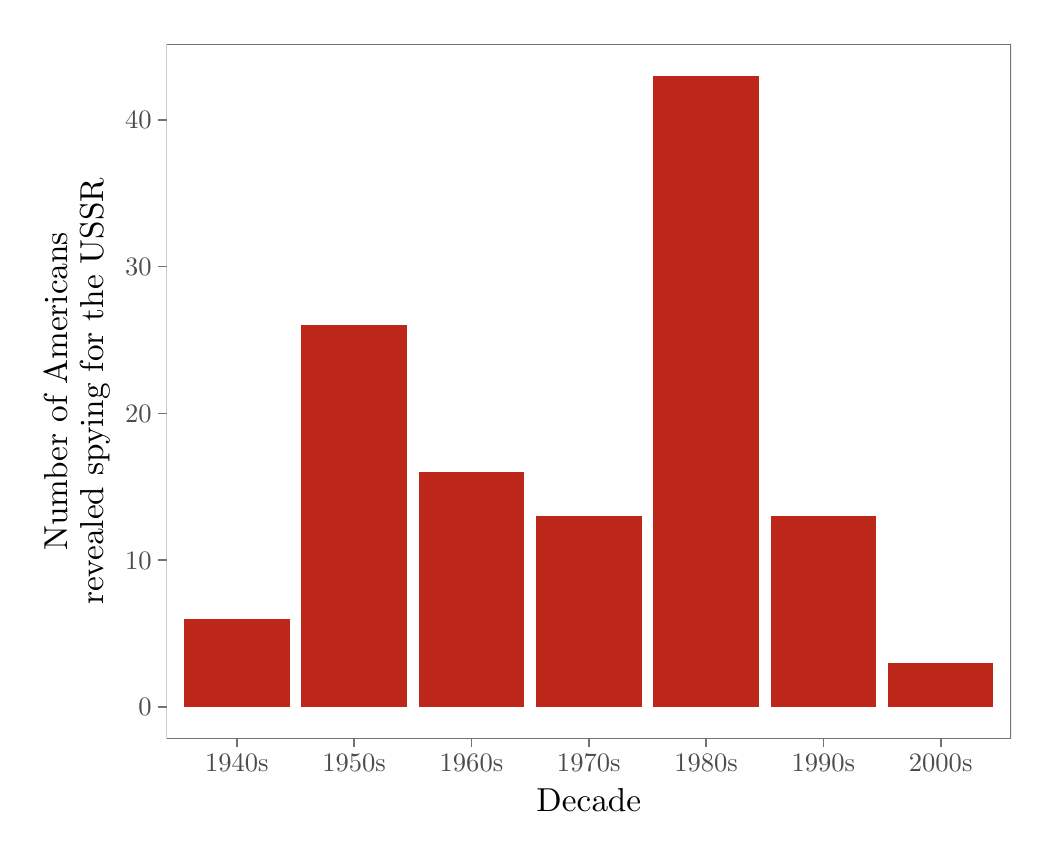
\begin{tikzpicture}[x=1pt,y=1pt]
\definecolor{fillColor}{RGB}{255,255,255}
\path[use as bounding box,fill=fillColor,fill opacity=0.00] (0,0) rectangle (361.35,289.08);
\begin{scope}
\path[clip] (  0.00,  0.00) rectangle (361.35,289.08);
\definecolor{drawColor}{RGB}{255,255,255}
\definecolor{fillColor}{RGB}{255,255,255}

\path[draw=drawColor,line width= 0.6pt,line join=round,line cap=round,fill=fillColor] (  0.00,  0.00) rectangle (361.35,289.08);
\end{scope}
\begin{scope}
\path[clip] ( 50.17, 32.28) rectangle (355.35,283.08);
\definecolor{fillColor}{RGB}{255,255,255}

\path[fill=fillColor] ( 50.17, 32.28) rectangle (355.35,283.08);
\definecolor{fillColor}{RGB}{188,39,26}

\path[fill=fillColor] ( 56.52, 43.68) rectangle ( 94.67, 75.49);

\path[fill=fillColor] ( 98.91, 43.68) rectangle (137.06,181.54);

\path[fill=fillColor] (141.30, 43.68) rectangle (179.45,128.51);

\path[fill=fillColor] (183.68, 43.68) rectangle (221.83,112.61);

\path[fill=fillColor] (226.07, 43.68) rectangle (264.22,271.68);

\path[fill=fillColor] (268.46, 43.68) rectangle (306.61,112.61);

\path[fill=fillColor] (310.84, 43.68) rectangle (348.99, 59.58);
\definecolor{drawColor}{gray}{0.45}

\path[draw=drawColor,line width= 0.6pt,line join=round,line cap=round] ( 50.17, 32.28) rectangle (355.35,283.08);
\end{scope}
\begin{scope}
\path[clip] (  0.00,  0.00) rectangle (361.35,289.08);
\definecolor{drawColor}{gray}{0.30}

\node[text=drawColor,anchor=base east,inner sep=0pt, outer sep=0pt, scale=  0.96] at ( 44.77, 40.37) {0};

\node[text=drawColor,anchor=base east,inner sep=0pt, outer sep=0pt, scale=  0.96] at ( 44.77, 93.39) {10};

\node[text=drawColor,anchor=base east,inner sep=0pt, outer sep=0pt, scale=  0.96] at ( 44.77,146.42) {20};

\node[text=drawColor,anchor=base east,inner sep=0pt, outer sep=0pt, scale=  0.96] at ( 44.77,199.44) {30};

\node[text=drawColor,anchor=base east,inner sep=0pt, outer sep=0pt, scale=  0.96] at ( 44.77,252.47) {40};
\end{scope}
\begin{scope}
\path[clip] (  0.00,  0.00) rectangle (361.35,289.08);
\definecolor{drawColor}{gray}{0.45}

\path[draw=drawColor,line width= 0.6pt,line join=round] ( 47.17, 43.68) --
	( 50.17, 43.68);

\path[draw=drawColor,line width= 0.6pt,line join=round] ( 47.17, 96.70) --
	( 50.17, 96.70);

\path[draw=drawColor,line width= 0.6pt,line join=round] ( 47.17,149.72) --
	( 50.17,149.72);

\path[draw=drawColor,line width= 0.6pt,line join=round] ( 47.17,202.75) --
	( 50.17,202.75);

\path[draw=drawColor,line width= 0.6pt,line join=round] ( 47.17,255.77) --
	( 50.17,255.77);
\end{scope}
\begin{scope}
\path[clip] (  0.00,  0.00) rectangle (361.35,289.08);
\definecolor{drawColor}{gray}{0.45}

\path[draw=drawColor,line width= 0.6pt,line join=round] ( 75.60, 29.28) --
	( 75.60, 32.28);

\path[draw=drawColor,line width= 0.6pt,line join=round] (117.98, 29.28) --
	(117.98, 32.28);

\path[draw=drawColor,line width= 0.6pt,line join=round] (160.37, 29.28) --
	(160.37, 32.28);

\path[draw=drawColor,line width= 0.6pt,line join=round] (202.76, 29.28) --
	(202.76, 32.28);

\path[draw=drawColor,line width= 0.6pt,line join=round] (245.14, 29.28) --
	(245.14, 32.28);

\path[draw=drawColor,line width= 0.6pt,line join=round] (287.53, 29.28) --
	(287.53, 32.28);

\path[draw=drawColor,line width= 0.6pt,line join=round] (329.92, 29.28) --
	(329.92, 32.28);
\end{scope}
\begin{scope}
\path[clip] (  0.00,  0.00) rectangle (361.35,289.08);
\definecolor{drawColor}{gray}{0.30}

\node[text=drawColor,anchor=base,inner sep=0pt, outer sep=0pt, scale=  0.96] at ( 75.60, 20.26) {1940s};

\node[text=drawColor,anchor=base,inner sep=0pt, outer sep=0pt, scale=  0.96] at (117.98, 20.26) {1950s};

\node[text=drawColor,anchor=base,inner sep=0pt, outer sep=0pt, scale=  0.96] at (160.37, 20.26) {1960s};

\node[text=drawColor,anchor=base,inner sep=0pt, outer sep=0pt, scale=  0.96] at (202.76, 20.26) {1970s};

\node[text=drawColor,anchor=base,inner sep=0pt, outer sep=0pt, scale=  0.96] at (245.14, 20.26) {1980s};

\node[text=drawColor,anchor=base,inner sep=0pt, outer sep=0pt, scale=  0.96] at (287.53, 20.26) {1990s};

\node[text=drawColor,anchor=base,inner sep=0pt, outer sep=0pt, scale=  0.96] at (329.92, 20.26) {2000s};
\end{scope}
\begin{scope}
\path[clip] (  0.00,  0.00) rectangle (361.35,289.08);
\definecolor{drawColor}{RGB}{1,2,2}

\node[text=drawColor,anchor=base,inner sep=0pt, outer sep=0pt, scale=  1.20] at (202.76,  6.00) {Decade};
\end{scope}
\begin{scope}
\path[clip] (  0.00,  0.00) rectangle (361.35,289.08);
\definecolor{drawColor}{RGB}{1,2,2}

\node[text=drawColor,rotate= 90.00,anchor=base,inner sep=0pt, outer sep=0pt, scale=  1.20] at ( 14.26,157.68) {Number of Americans };

\node[text=drawColor,rotate= 90.00,anchor=base,inner sep=0pt, outer sep=0pt, scale=  1.20] at ( 27.22,157.68) {revealed spying for the USSR};
\end{scope}
\end{tikzpicture}

  \label{decade_spies}
  \caption{Number of Americans alleged to be spying for the USSR, by decade}
\end{figure}

Two things should immediately stand out about this table.
The first is that a lot of espionage is taking place against the United States during the Cold War, specifically by the USSR.

Second is upticks in the 1950s and 1980s

Herbig says the uptick in the 1980s a result of better enforcement, not more spies.\footcite{herbig_espionage_2002}

That most of these cases are essentially ignored diplomatically is a strong argument in favor of my point that the diplomatic impact of espionage is routinely minimized.

Here's a few cases that weren't ignored, brief summary of their damage, and the diplomatic consequences. Unclear if this merits its own section, or should get folded into general analysis.

Kim Philby - Brit who spied then successfully defected to USSR

Oleg Penkovsky - Soviet citizen turned American agent, executed

John Walker - American citizen turned Soviet agent, imprisoned

Oleg Gordievsky - KGB officer turned British agent, successfully defected
% 1971 mass expulsion from Britain

\section{Appendix}
\subsection{List of Alleged American Spies}
\begin{multicols}{2}
\setlength{\parindent}{0ex}
Laurence Duggan (1948)\newline
Judith Coplon (1949)\newline
Gustav Adolph Mueller (1949)\newline
Joel Barr (1950)\newline
Harry Gold (1950)\newline
David Greenglass (1950)\newline
Ruth Greenglass (1950)\newline
Russell McNutt (1950)\newline
Miriam Moskowitz (1950)\newline
Ethel Grecnglass Rosenberg (1950)\newline
Julius Rosenberg (1950)\newline
Alfred Epaminondas Sarant (1950)\newline
Morton Sobell (1950)\newline
William Wcisband (1950)\newline
William W. Remington (1951)\newline
Robert Lee Johnson (1953)\newline
James Allen Mintkenbaugh (1953)\newline
Kurt Leopold Ponger (1953)\newline
Otto Verber (1953)\newline
Jacob Abram (1957)\newline
George Holmes French (1957)\newline
Boris Morros (1957)\newline
Jack Soble (1957)\newline
Myra Soble (1957)\newline
Robert Soblen (1957)\newline
Alfred Stern (1957)\newline
Martha Stern (1957)\newline
Jane Foster Zlatovski (1957)\newline
Roy Adair Rhodes (1958)\newline
John Gilmore (1960)\newline
William Hamilton Martin (1960)\newline
Bernon Ferguson Mitchell (1960)\newline
John William Butenko (1963)\newline
Nelson Cornelious Drummond (1963)\newline
Jack Edward Dunlap (1963)\newline
Victor Norris Hamilton (1963)\newline
First name unknown Wesson (1963)\newline
George John Gessner (1964)\newline
Robert Glenn Thompson (1965)\newline
Herbert Boeckenhaupt (1966)\newline
William Henry Whalcn (1966)\newline
Ulysses Leonard Harris (1967)\newline
Gary Lee Ledbetter (1967)\newline
Leonard JenkinssTSaf-ford (1967)\newline
Edward Hillcdon Winc (1968)\newline
Raymond George DeChamplin (1971)\newline
Walter Thomas Perkins (1971)\newline
First name unknown Walton (1972)\newline
Oliver Everett Grunden (1973)\newline
james David Wood (1973)\newline
Sadag Katcher Dedeyan (1975)\newline
Edwin Gibbons Moore II (1975)\newline
Sarkis Paskalian (1975)\newline
David Henry Barnett (1977)\newline
Christopher Boyce (1977)\newline
Andrew Daulton Lee (1977)\newline
Ivan Rogalsky (1977)\newline
William Kampiles (1978)\newline
Glenn Michael Souther (1980)\newline
Chrisropher Michael Cooke (1981)\newline
Joseph George Hclmich (1981)\newline
Michael Richard Murphy (1981)\newline
Brian Patrick Horton (1982)\newline
Brian Everett Sluvens (1982)\newline
Robert Wade Ellis (1983)\newline
Jeffery Loring Pickering (1983)\newline
Hans Palmer Wold (1983)\newline
Thomas Patrick Cavanaugh (1984)\newline
Robert Ernest Cordrey (1984)\newline
Richard William Miller (1984)\newline
Nikolai Ogorodnikov (1984)\newline
Svetlana Ogorodnikov (1984)\newline
Charles Dale Slatten (1984)\newline
Richard Craig Smith (1984)\newline
Edward Owen Buchanan (1985)\newline
Dale Vern Irene (1985)\newline
Randy Miles Jeffries (1985)\newline
Ronald William Pelton (1985)\newline
Francis Xavier Pizzo (1985)\newline
Bruce Edward Tobias (1985)\newline
Michael Timothy Tobias (1985)\newline
Arthur James Walker (1985)\newline
Michael Lance Walker (1985)\newline
John Anthony Walker Jr. (1985)\newline
Jerry Alfred Whitworth (1985)\newline
Arnold Bracy (1986)\newline
Robert Dean Hagucwood (1986)\newline
Edward Lee Howard (1986)\newline
Clayton John Lonetrre (1986)\newline
Bruce Damian Ott (1986)\newline
Svetlana Tumanova (1987)\newline
James Michael Hall III (1988)\newline
Daniel Walter Richardson (1988)\newline
Huscyin Yildirim (1988)\newline
Russell Paul Brown (1989)\newline
John Joseph Haeger (1989)\newline
Craig D. Kunkle (1989)\newline
Frank Arnold Ncsbitt (1989)\newline
Charles Edward Schoof (1989)\newline
James Rodney Wilmoth (1989)\newline
Ronald Craig WolfMay S (1989)\newline
Felix Bloch (1990)\newline
Aldrich Hazen Ames (1994)\newline
Maria del Rosario Casa Ames (1994)\newline
Patricia Lipka (1994)\newline
Robert Stephen Lipka (1994)\newline
Kota Subrahmanyam (1995)\newline
Robert P. Hanssen (1996)\newline
Kurt G. Lessenthien (1996)\newline
Harold ]. Nicholson (1996)\newline
Nathaniel Nicholson (1996)\newline
Edwin Earl Pitts (1996)\newline
David Sheldon Boone (1998)\newline
Daniel M. King (1999)\newline
George Trofimoff (2000)\newline
Hafiz Ahmad Ali Shaaban (2005)\newline
Ariel Jonathan Wcinmann (2006)\newline
Robert Patrick Hoffman (2012)
\end{multicols}


\newpage
\printbibliography[heading=subbibliography]

\end{refsegment}
1\end{document}
